\documentclass[11pt]{exam}
\RequirePackage{amssymb, amsfonts, amsmath, latexsym, verbatim, xspace, setspace}
\RequirePackage{tikz, pgflibraryplotmarks}
\usepackage[margin=1in]{geometry}
\usepackage{float}

\newcommand{\class}{Math 1234}
\newcommand{\term}{Spring 2012}
\newcommand{\examnum}{Exam 2}
\newcommand{\examdate}{Today}
\newcommand{\timelimit}{50 Minutes}

\singlespacing
% \onehalfspacing
% \doublespacing

\parindent 0ex

\begin{document} 
\pagestyle{head}
\firstpageheader{}{}{}
\runningheader{\class}{\examnum\ - Page \thepage\ of \numpages}{\examdate}
\runningheadrule

\begin{flushright}
\begin{tabular}{p{2.8in} r l}
\textbf{\class} & \textbf{Name (Print):} & \makebox[2in]{\hrulefill}\\
\textbf{\term} &&\\
\textbf{\examnum} &&\\
\textbf{Time Limit: \timelimit}
\end{tabular}\\
\end{flushright}
\rule[1ex]{\textwidth}{.1pt}


This exam contains \numpages\ pages (including this cover page) and
\numquestions\ problems.  Check to see if any pages are missing.  Enter
all requested information on the top of this page, and put your initials
on the top of every page, in case the pages become separated.\\

You may \textit{not} use your books, notes, or any calculator on this exam.\\

You are required to show your work on each problem on this exam.  The following rules apply:\\

\begin{minipage}[t]{3.7in}
\vspace{0pt}
\begin{itemize}

\item \textbf{If you use a ``fundamental theorem'' you must indicate this} and explain
why the theorem may be applied.

\item \textbf{Organize your work}, in a reasonably neat and coherent way, in
the space provided. Work scattered all over the page without a clear ordering will 
receive very little credit.  

\item \textbf{Mysterious or unsupported answers will not receive full
credit}.  A correct answer, unsupported by calculations, explanation,
or algebraic work will receive no credit; an incorrect answer supported
by substantially correct calculations and explanations might still receive
partial credit.


\item If you need more space, use the back of the pages; clearly indicate when you have done this.
\end{itemize}
\end{minipage}
\hfill

\newpage 


\begin{questions}

% Basic question
%\addpoints
%\question[10] |
%\newpage

% Basic question
%\addpoints
%\question[10] |

% Question with parts
%\newpage
%\addpoints
%\question |
%\begin{parts}
%\part[5] |
%\vfill
%\part[5] |
%\vfill
%\end{parts}

%\newpage
%\addpoints
%\question[10] |
%\noaddpoints % If you remove this line, the grading table will show 20 points for this problem.
%\begin{parts}
%\part[5] |
%\vspace{4.5in}
%\part[5] |
%\end{parts}
\addpoints
\question[10] Figure 21-11 shows four situations in which five charged particles are evenly spaced along an axis. The charge values are indicated except for the central particle, which has the same charge in all four situations. Rank the situations according to the magnitude of the net electrostatic force on the central particle, greatest first.\begin{figure}[H]
\centering
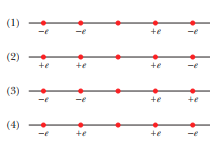
\includegraphics[scale=0.8]{assets/Halliday_ch21q1.png}
\end{figure}
\newpage

\addpoints
\question[10] Figure 21-12 shows three pairs of identical spheres that are to be touched together and then separated. The initial charges on them are indicated. Rank the pairs according to (a) the magnitude of the charge transferred during touching and (b)  the charge left on the positively charged sphere, greatest first.\begin{figure}[H]
\centering
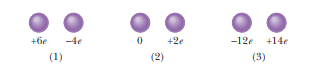
\includegraphics[scale=0.8]{assets/Halliday_ch21q2.png}
\end{figure}
\newpage

\addpoints
\question[10] Figure 21-13 shows four situations in which charged particles are fixed in place on an axis. In which situations is there a point to the left of the particles where an electron will be in equilibrium?\begin{figure}[H]
\centering
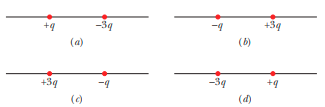
\includegraphics[scale=0.8]{assets/Halliday_ch21q3.png}
\end{figure}
\newpage

\addpoints
\question[10] Figure 21-14 shows two charged particles on an axis. The charges are free to move. However, a third charged particle can be placed at a certain point such that all three particles are then in equilibrium. (a) Is that point to the left of the first two particles, to their right, or between them? (b) Should the third particle be positively or negatively charged? (c)  Is the equilibrium stable or unstable?\begin{figure}[H]
\centering
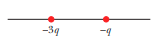
\includegraphics[scale=0.8]{assets/Halliday_ch21q4.png}
\end{figure}
\newpage

\addpoints
\question[10] In Fig. 21-15, a central particle of charge -q is surrounded by two circular rings of charged particles. What are the magnitude and direction of the net electrostatic force on the central particle due to the other particles? (Hint - Consider symmetry.)\begin{figure}[H]
\centering
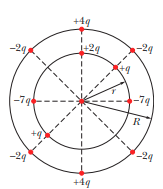
\includegraphics[scale=0.8]{assets/Halliday_ch21q5.png}
\end{figure}
\newpage

\addpoints
\question[10] In Fig. 21-26, particle 1 of charge +1.0 $\mu$ C and particle  2 of charge -3.0 $\mu$ C are held at separation L = 10.0 cm on an x axis. If particle 3 of unknown charge q3 is to be located such that the net electrostatic force on it from particles 1 and 2 is zero, what must be the (a) x and (b) y coordinates of particle 3?\begin{figure}[H]
\centering
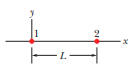
\includegraphics[scale=0.8]{assets/Halliday_ch21p13.png}
\end{figure}
\newpage





\end{questions}
\end{document}